\section{Experiments}

We evaluate PEC-Nav through four analyses. A contextual positioning against published results, ablations isolating each component and each feedback path, a direct measurement of calibration behaviour, and an analysis of cost and failure modes.

\subsection{Setup}
\label{sec:setup}

\paragraph{Dataset.} All experiments use LMEE-Benchmark dataset official 58-task evaluation subset~\cite{wang2026memoryexplorer}, comprising 32 HM3D scenes, 274 navigation goals and 145 QA questions, stratified into easy, medium and hard by region count, goal count and distance. We adopt the benchmark unchanged and use its Qwen2.5-VL-7B~\cite{bai2025qwen25vl} QA model as our backend, which holds the answering stage constant across our ablations so differences there originate in what search delivered. It does not make our pipeline equivalent to the reference system, whose memory module differs.

\paragraph{Units and metrics.} An episode is one LMEE-Benchmark dataset~\cite{wang2026memoryexplorer} task containing several navigation subtasks, one per goal in its instruction, giving 274 subtasks over 58 episodes. Navigation metrics are per subtask, so every $N$ below counts subtasks. Success Rate (\textbf{SR}) is the fraction reaching the target within 1.0\,m, and Success weighted by Path Length (\textbf{SPL})~\cite{anderson2018spl} weights success by path efficiency on a 0 to 100 scale. Open-ended answers use \textbf{MLLM-Score}~\cite{wang2026memoryexplorer}, multiple choice uses \textbf{accuracy}. An episode is a success if all its subtasks succeed, partial if some do, and fail if none. Instrumentation coverage differs by analysis, with correction logs retained for 29 episodes and failure logs for 36 across 19 scenes, so figures drawn from them describe the mechanism rather than the full set.

\paragraph{Protocol.} Goal extraction and search reasoning use GPT-4o~\cite{openai2024gpt4o} via API. Memory-based question answering runs locally on the benchmark's own Qwen2.5-VL-7B~\cite{bai2025qwen25vl} model in bf16 on a single NVIDIA RTX 3090, loaded only for QA subtasks. Search reasoning depends on a hosted model versioned outside our control, so reproduction requires the same snapshot and we report single runs. Comparison rows are quoted from the benchmark paper and assume its protocol and step budget, treating an instruction's named objects as successive subtasks. Our counts recover 274 subtasks against 272 for those rows, so per-split percentages are comparable to within roughly 0.4 points and no finer.

\subsection{Comparison on the LMEE-Benchmark dataset}

\begin{table*}[htbp]
\centering
\caption{\textbf{Results on the LMEE-Benchmark dataset.} Upper block is retrieval-augmented QA over memory banks collected post-exploration, lower block is active exploration.}
\label{tab:lmee}
\footnotesize
\setlength{\tabcolsep}{3pt}
\begin{tabular}{l|cccc|cccc|cccc|cccc}
\toprule
& \multicolumn{4}{|c}{\textbf{Easy}} & \multicolumn{4}{|c}{\textbf{Medium}} & \multicolumn{4}{|c}{\textbf{Hard}} & \multicolumn{4}{|c}{\textbf{Total}} \\
\cmidrule(lr){2-5} \cmidrule(lr){6-9} \cmidrule(lr){10-13} \cmidrule(lr){14-17}
& \multicolumn{2}{c}{Nav} & \multicolumn{2}{c|}{QA} & \multicolumn{2}{c}{Nav} & \multicolumn{2}{c|}{QA} & \multicolumn{2}{c}{Nav} & \multicolumn{2}{c|}{QA} & \multicolumn{2}{c}{Nav} & \multicolumn{2}{c}{QA} \\
\cmidrule(lr){2-3} \cmidrule(lr){4-5} \cmidrule(lr){6-7} \cmidrule(lr){8-9} \cmidrule(lr){10-11} \cmidrule(lr){12-13} \cmidrule(lr){14-15} \cmidrule(lr){16-17}
\textbf{Method} & SR & SPL & Score & Acc & SR & SPL & Score & Acc & SR & SPL & Score & Acc & SR & SPL & Score & Acc \\
\midrule
\multicolumn{17}{l}{\emph{Retrieval-Augmented QA}} \\
LLaVA-OneVision-7B~\cite{li2024llavaov} & N/A & N/A & 35.71 & 57.14 & N/A & N/A & 42.02 & 62.77 & N/A & N/A & 25.00 & 43.75 & N/A & N/A & 38.62 & 59.31 \\
Llama3.2-Vision-11B & N/A & N/A & 43.57 & 48.57 & N/A & N/A & 28.19 & 37.23 & N/A & N/A & 20.31 & 31.25 & N/A & N/A & 31.03 & 39.31 \\
Qwen2.5-VL-7B~\cite{bai2025qwen25vl} & N/A & N/A & 36.43 & 65.71 & N/A & N/A & 43.62 & 53.19 & N/A & N/A & 42.19 & 43.75 & N/A & N/A & 41.72 & 55.17 \\
InternVL3-8B & N/A & N/A & 42.14 & 65.71 & N/A & N/A & 41.22 & 54.26 & N/A & N/A & 26.56 & 43.75 & N/A & N/A & 39.83 & 55.86 \\
Qwen3-VL-8B~\cite{bai2025qwen3} & N/A & N/A & 43.57 & 65.71 & N/A & N/A & 36.70 & 58.51 & N/A & N/A & 32.81 & 62.50 & N/A & N/A & 37.93 & 60.69 \\
GPT-4o~\cite{openai2024gpt4o} & N/A & N/A & 43.57 & 65.71 & N/A & N/A & 37.50 & 51.06 & N/A & N/A & 40.62 & 56.25 & N/A & N/A & 39.31 & 55.17 \\
Gemini-2.5-Flash & N/A & N/A & 44.29 & 51.43 & N/A & N/A & 37.77 & 50.00 & N/A & N/A & 23.44 & 50.00 & N/A & N/A & 37.76 & 50.34 \\
\midrule
\multicolumn{17}{l}{\emph{MLLM Exploration}} \\
Explore-EQA~\cite{ren2024exploreeqa} & 4.26 & 4.26 & N/A & N/A & 15.17 & 8.67 & N/A & N/A & 14.89 & 7.25 & N/A & N/A & 13.24 & 7.66 & N/A & N/A \\
3D-Mem~\cite{huang20243dmem} & 21.28 & 9.68 & 30.71 & 42.86 & 15.73 & 6.09 & 34.57 & 44.68 & 17.02 & 6.97 & 25.00 & 18.75 & 16.91 & 6.86 & 32.59 & 41.38 \\
RA-Mem$^{\ddagger}$~\cite{wang2026memoryexplorer} & 25.53 & 15.65 & 34.29 & 54.29 & \textbf{21.35} & 12.14 & 37.77 & 62.77 & 14.89 & 8.86 & 25.00 & 43.75 & 20.96 & 12.18 & 35.52 & 58.62 \\
MemoryExplorer~\cite{wang2026memoryexplorer} & 31.91 & 21.11 & 35.71 & \textbf{68.57} & \textbf{21.35} & 14.03 & 48.14 & 63.83 & 23.40 & 12.51 & 34.38 & \textbf{68.75} & 23.53 & 14.99 & 43.62 & 65.52 \\
\midrule
\textbf{PEC-Nav (Ours)} & \textbf{40.43} & \textbf{25.06} & \textbf{48.57} & \textbf{68.57} & 20.11 & \textbf{14.35} & \textbf{62.77} & \textbf{67.02} & \textbf{25.00} & \textbf{18.21} & \textbf{50.00} & 56.25 & \textbf{24.45} & \textbf{16.86} & \textbf{57.93} & \textbf{66.21} \\
\bottomrule
\end{tabular}
\end{table*}

Table~\ref{tab:lmee} places PEC-Nav among results from the available literature, reporting MLLM-Score for open-ended answers and accuracy for multiple choice, with bold marking the best value per column and N/A a metric a method does not produce. Navigation columns are compared over the exploration block, since retrieval-augmented methods answer from memory banks collected beforehand and perform no navigation. RA-Mem~\cite{wang2026memoryexplorer}, marked $\ddagger$, is a retrieval-augmented variant of 3D-Mem~\cite{huang20243dmem} introduced as a baseline alongside the benchmark. On the \emph{Total} column it reaches 24.45\% SR, 16.86 SPL, 57.93 MLLM-Score and 66.21\% QA accuracy, ahead of MemoryExplorer~\cite{wang2026memoryexplorer} on SR, SPL and MLLM-Score. The largest per-column margin is MLLM-Score on \emph{Hard} at 50.00 against 34.38, followed by \emph{Medium}. The picture is not uniform. MemoryExplorer retains the better SR on \emph{Medium} and the better QA accuracy on \emph{Hard}, where Qwen3-VL-8B~\cite{bai2025qwen3} also exceeds us, and Easy and Total QA accuracy read as ties. The gains are therefore in navigation and open-ended answer quality rather than multiple-choice accuracy, where the fixed QA module dominates.

\subsection{Ablation Studies}
\label{sec:ablations}

\begin{table}[htbp]
\centering
\caption{\textbf{Feedback-path ablation} over 47 navigation subtasks.}
\label{tab:feedback}
\footnotesize
\setlength{\tabcolsep}{3pt}
\begin{tabular}{@{}l|cc|ccc@{}}
\toprule
\textbf{Variant} & $\sigma_t$ & $w_e,w_g$ & \textbf{SR} $\uparrow$ & \textbf{SPL} $\uparrow$ & $\Delta$\textbf{SR} \\
\midrule
No correction & \xmark & \xmark & 36.17 \,\scriptsize(17/47) & 20.75 & --- \\
Confidence only & \cmark & \xmark & 40.43 \,\scriptsize(19/47) & 25.57 & +4.26 \\
Reweighting only & \xmark & \cmark & 36.17 \,\scriptsize(17/47) & 22.09 & +0.00 \\
\textbf{Full PEC loop} & \cmark & \cmark & \textbf{40.43} \,\scriptsize(19/47) & \textbf{28.38} & \textbf{+4.26} \\
\bottomrule
\end{tabular}
\end{table}

\paragraph{Isolating the correction phase.} The first and last rows of Table~\ref{tab:feedback} differ only in whether arrival detection fires. With correction disabled the predictor still runs and predictions are still stored, but surprise is never computed, so $\sigma_t$ never updates and the weights never shift, leaving the agent with strictly more computation and no adaptation. Enabling correction raises SR from 36.17\% to 40.43\% and SPL from 20.75 to 28.38.

In absolute terms the SR change is 17 successes against 19, and the two proportions are indistinguishable on an unpaired reading, with Wilson 95\% intervals of $[24.0, 50.5]$ and $[27.6, 54.7]$ and Fisher exact $p = 0.83$. The design is paired, but we did not log per-subtask outcome pairs and so decline to quote McNemar's test. The 37\% relative gain in SPL is the more informative number, and does not depend on a success threshold. One subtask is worth 2.13 SR points at $N = 47$ and 4.17 at $N = 24$.

\begin{table}[htbp]
\centering
\caption{\textbf{Component ablation} over 24 navigation subtasks, with success counts in parentheses.}
\label{tab:ablation_all}
\footnotesize
\setlength{\tabcolsep}{3pt}
\begin{tabular}{@{}l|cccc@{}}
\toprule
\textbf{Configuration} & \textbf{SR (\%)} $\uparrow$ & \textbf{SPL} $\uparrow$ & \textbf{N} & $\Delta$\textbf{SR} \\
\midrule
Static baseline & 54.17 \,\scriptsize(13/24) & 34.35 & 24 & --- \\
\quad + Goal extraction & 54.17 \,\scriptsize(13/24) & 36.05 & 24 & 0.00 \\
\quad + Semantic predictor & 50.00 \,\scriptsize(12/24) & 32.36 & 24 & $-$4.17 \\
\quad \textbf{+ Online correction (full)} & \textbf{58.33} \,\scriptsize(14/24) & \textbf{41.47} & 24 & \textbf{+4.16} \\
\bottomrule
\end{tabular}
\end{table}

\paragraph{Component ablation.} Table~\ref{tab:ablation_all} adds each component cumulatively over a separate 2-scene subset, where one subtask is worth 4.17 SR points and the SPL column therefore carries more of the signal. Absolute values are not comparable with Table~\ref{tab:feedback}, since the static baseline scores 54.17 here against 36.17 there, so these rows are within-table contrasts only. Goal extraction leaves SR unchanged and lifts SPL from 34.35 to 36.05. Adding the semantic predictor then moves SR by $-4.17$ and SPL by $-3.69$, which indicates that an uncalibrated predictor steers the agent toward frontiers matching its prediction rather than the observation. Correction recovers that loss and clears the baseline, moving SR by $+8.33$ and SPL by $+9.11$ over the predictor-only row. Within this table the gain is therefore attributable to the loop rather than the predictor, though at $N = 24$ that remains a hypothesis the data are consistent with.

\paragraph{Which feedback path carries the effect.} Surprise rescales predictor confidence through $\sigma_t$ and reweights the value function through $w_e$ and $w_g$. Table~\ref{tab:feedback} enables each independently over a 47-subtask ablation subset, and every nonzero SR difference in it is two subtasks. Confidence scaling recovers the full SR gain alone, while reweighting leaves SR unchanged and lifts SPL from 20.75 to 22.09. The full loop matches confidence-only on SR and extends SPL to 28.38, so reweighting contributes path efficiency rather than successes. Both arms succeed on 19 of 47 subtasks, and we have not verified they are the same 19, which is a further reason to read this table from its SPL column.

\subsection{Does the Agent Calibrate?}
\label{sec:pec-dynamics}

This section asks whether the mechanism behaves as claimed, using quantities from the correction logs.

\begin{figure}[htbp]
\centering
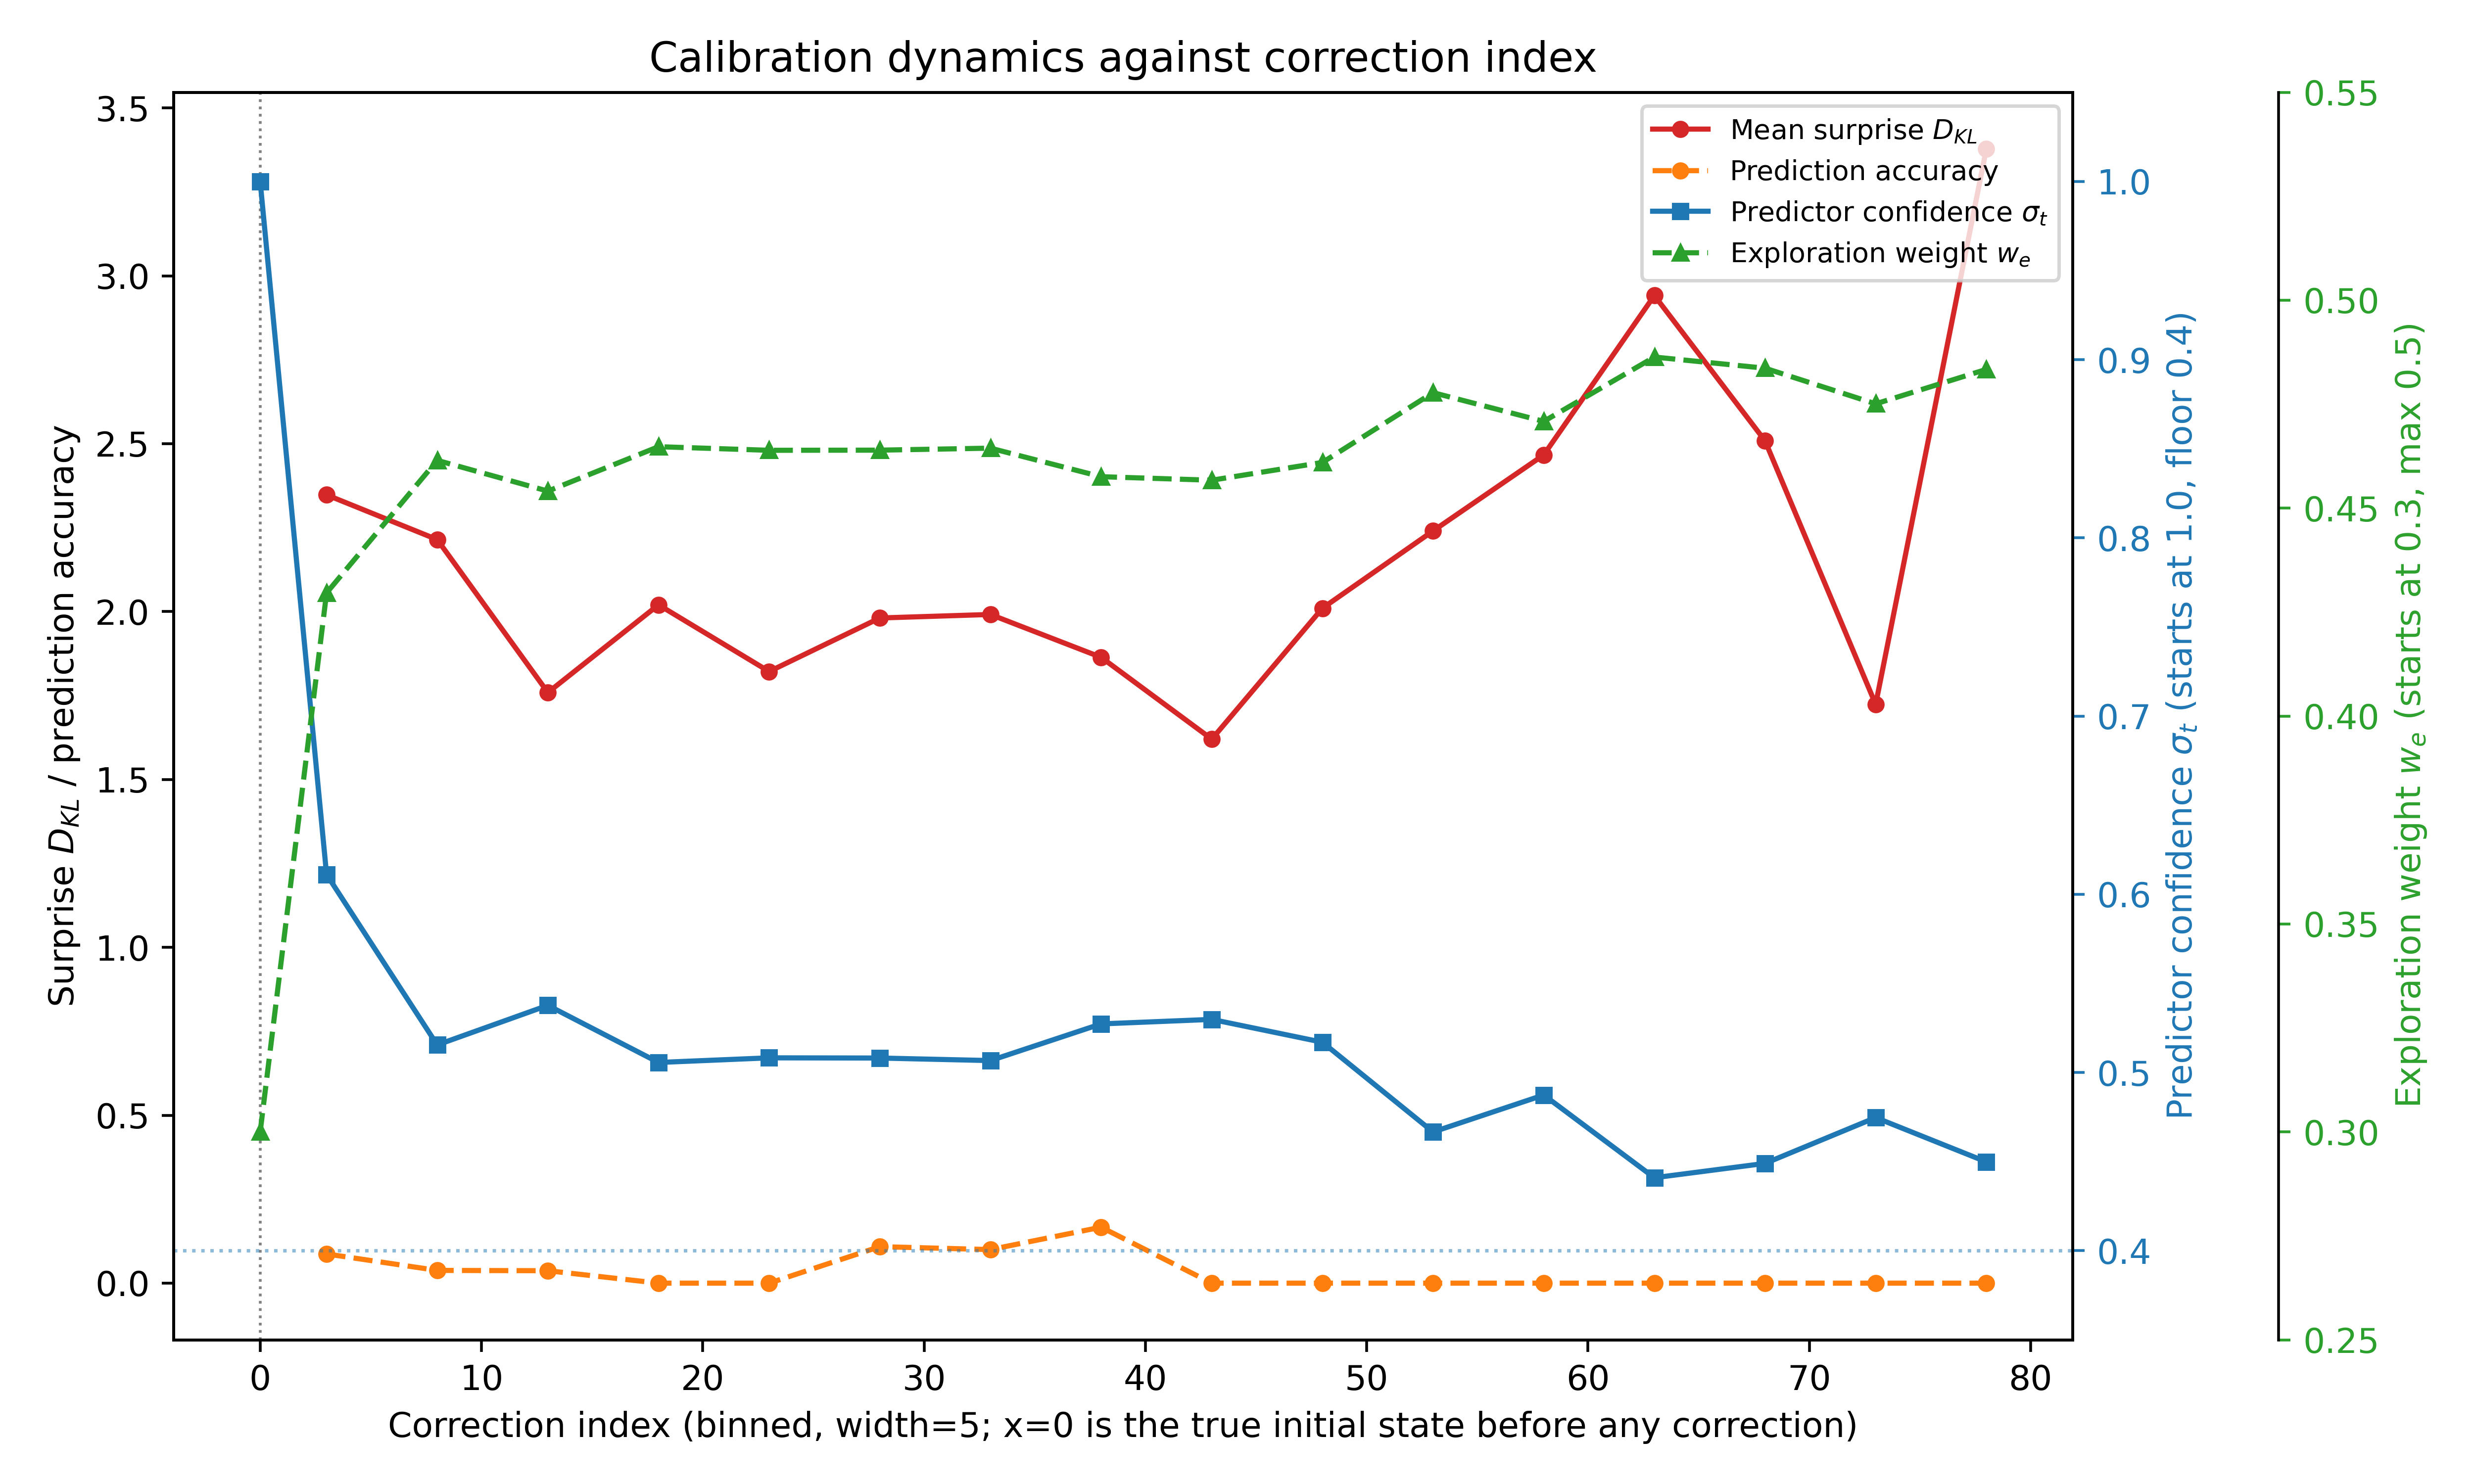
\includegraphics[width=0.88\linewidth]{figures/figure3.png}
\caption{Calibration dynamics: surprise, accuracy, uncertainty vs.\ correction index.}
\label{fig:calibration}
\end{figure}

The regime is the one the self-calibration design anticipates. Per-episode mean divergence is of order $2$, which puts $n_t$ near $0.86$ and $\sigma_t$ within roughly $0.08$ of its floor for most of an episode, so the controller commits quickly to a low-trust setting and holds there. Figure~\ref{fig:calibration} confirms this, with $\sigma_t$ falling and $w_e$ rising under sustained surprise. Neither surprise nor accuracy is expected to improve, since the predictor is never updated and the loop's role is to downweight it.

\begin{figure*}[htbp]
\centering
\includegraphics[width=0.85\textwidth]{figures/qualitative image pec .pdf}
\caption{\textbf{Qualitative examples of PEC-Nav.}}
\label{fig:qualitative}
\end{figure*}


\begin{figure}[htbp]
\centering
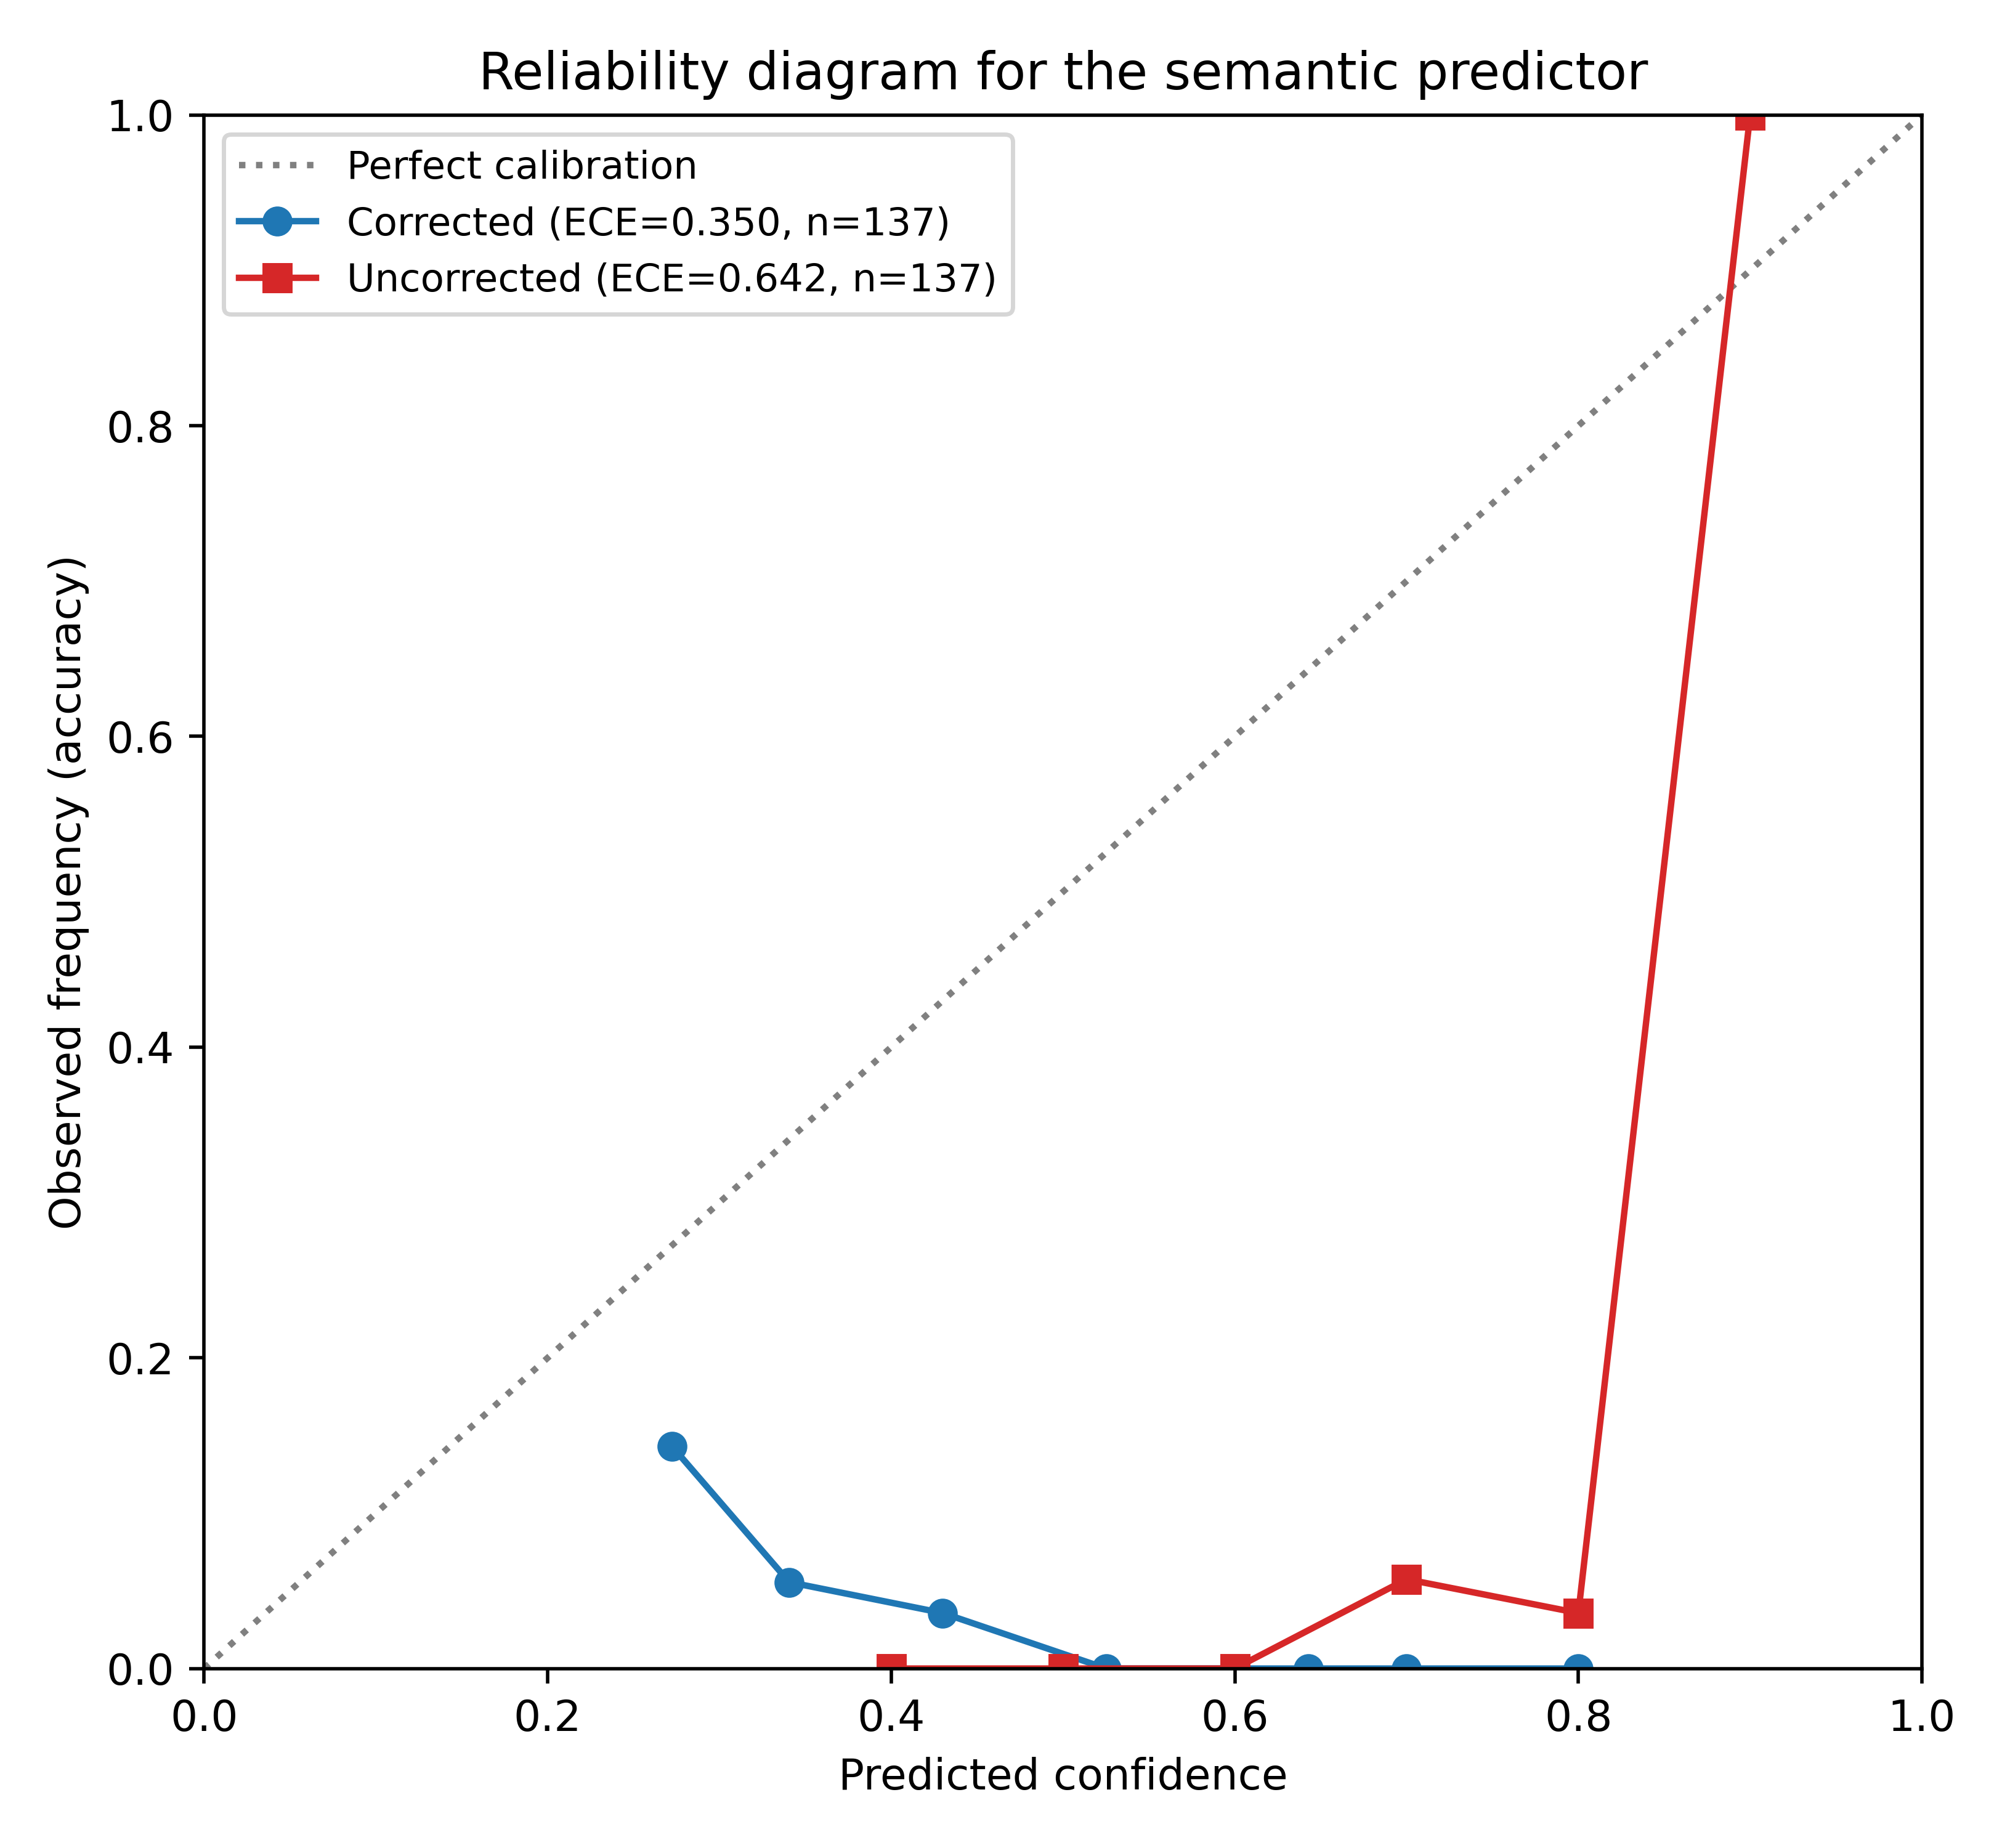
\includegraphics[width=0.75\linewidth]{figures/figure4.png}
\caption{Reliability diagram, with/without correction loop ($n=137$); ECE drops from $0.642$ to $0.350$.}
\label{fig:reliability}
\end{figure}

Figure~\ref{fig:reliability} makes the claim quantitative, and expected calibration error falls from $0.642$ to $0.350$. We are deliberate about what this shows. Since $\sigma_t$ is a multiplicative shrinkage on a systematically overconfident predictor, any downward rescaling moves the metric the same way, and the mechanism is self-referential in that the same $\sigma_t$ enters the divergence driving it. The figure establishes that the loop selects a shrinkage improving calibration without supervision, not that it beats a well-chosen constant, a control we did not run.

\subsection{Analysis}
\label{sec:analysis}

\paragraph{Surprise as a diagnostic.} Across the 29 episodes with retained correction logs, per-episode mean surprise is comparable between partial ($2.10$, $n = 13$) and failed ($1.92$, $n = 16$) episodes. That subset contains no fully successful episode, so the comparison that would matter most cannot be made on it. Surprise aggregated to the episode level is therefore not a reliable diagnostic, and the within-episode dynamics remain the operative signal.

\begin{table}[htbp]
\centering
\caption{\textbf{Cost of the correction loop}, per-episode averages, 4-scene subset.}
\label{tab:compute}
\footnotesize
\setlength{\tabcolsep}{3pt}
\begin{tabular}{@{}l|cc@{}}
\toprule
\textbf{Quantity (per episode)} & \textbf{Static baseline} & \textbf{PEC-Nav} \\
\midrule
VLM calls            & 144.1  & 227.7 \\
Navigation steps     & 100.3  & 95.6 \\
Wall-clock (s)       & 765.09 & 1160.92 \\
Peak GPU memory (GB) & 22.62  & 22.62 \\
\bottomrule
\end{tabular}
\end{table}

\paragraph{Cost of the loop.} Table~\ref{tab:compute} reports the loop's cost on the 4-scene subset, raising VLM calls by 58\% and wall-clock time by 52\%, borne almost entirely in hosted-API calls. The 83.6 extra calls per episode exceed the roughly 30 corrections fired, because each step prices a prediction for every open frontier, not only the one later verified. Peak GPU memory is unchanged, since only the shared local QA model occupies it, and navigation steps fall, so the added cost is deliberation rather than travel, which is also why SPL improves while compute rises. We report no compute figures for the comparison systems, so we claim only that the overhead is a bounded inference-time cost requiring no training and no additional local hardware.

\begin{figure}[htbp]
\centering
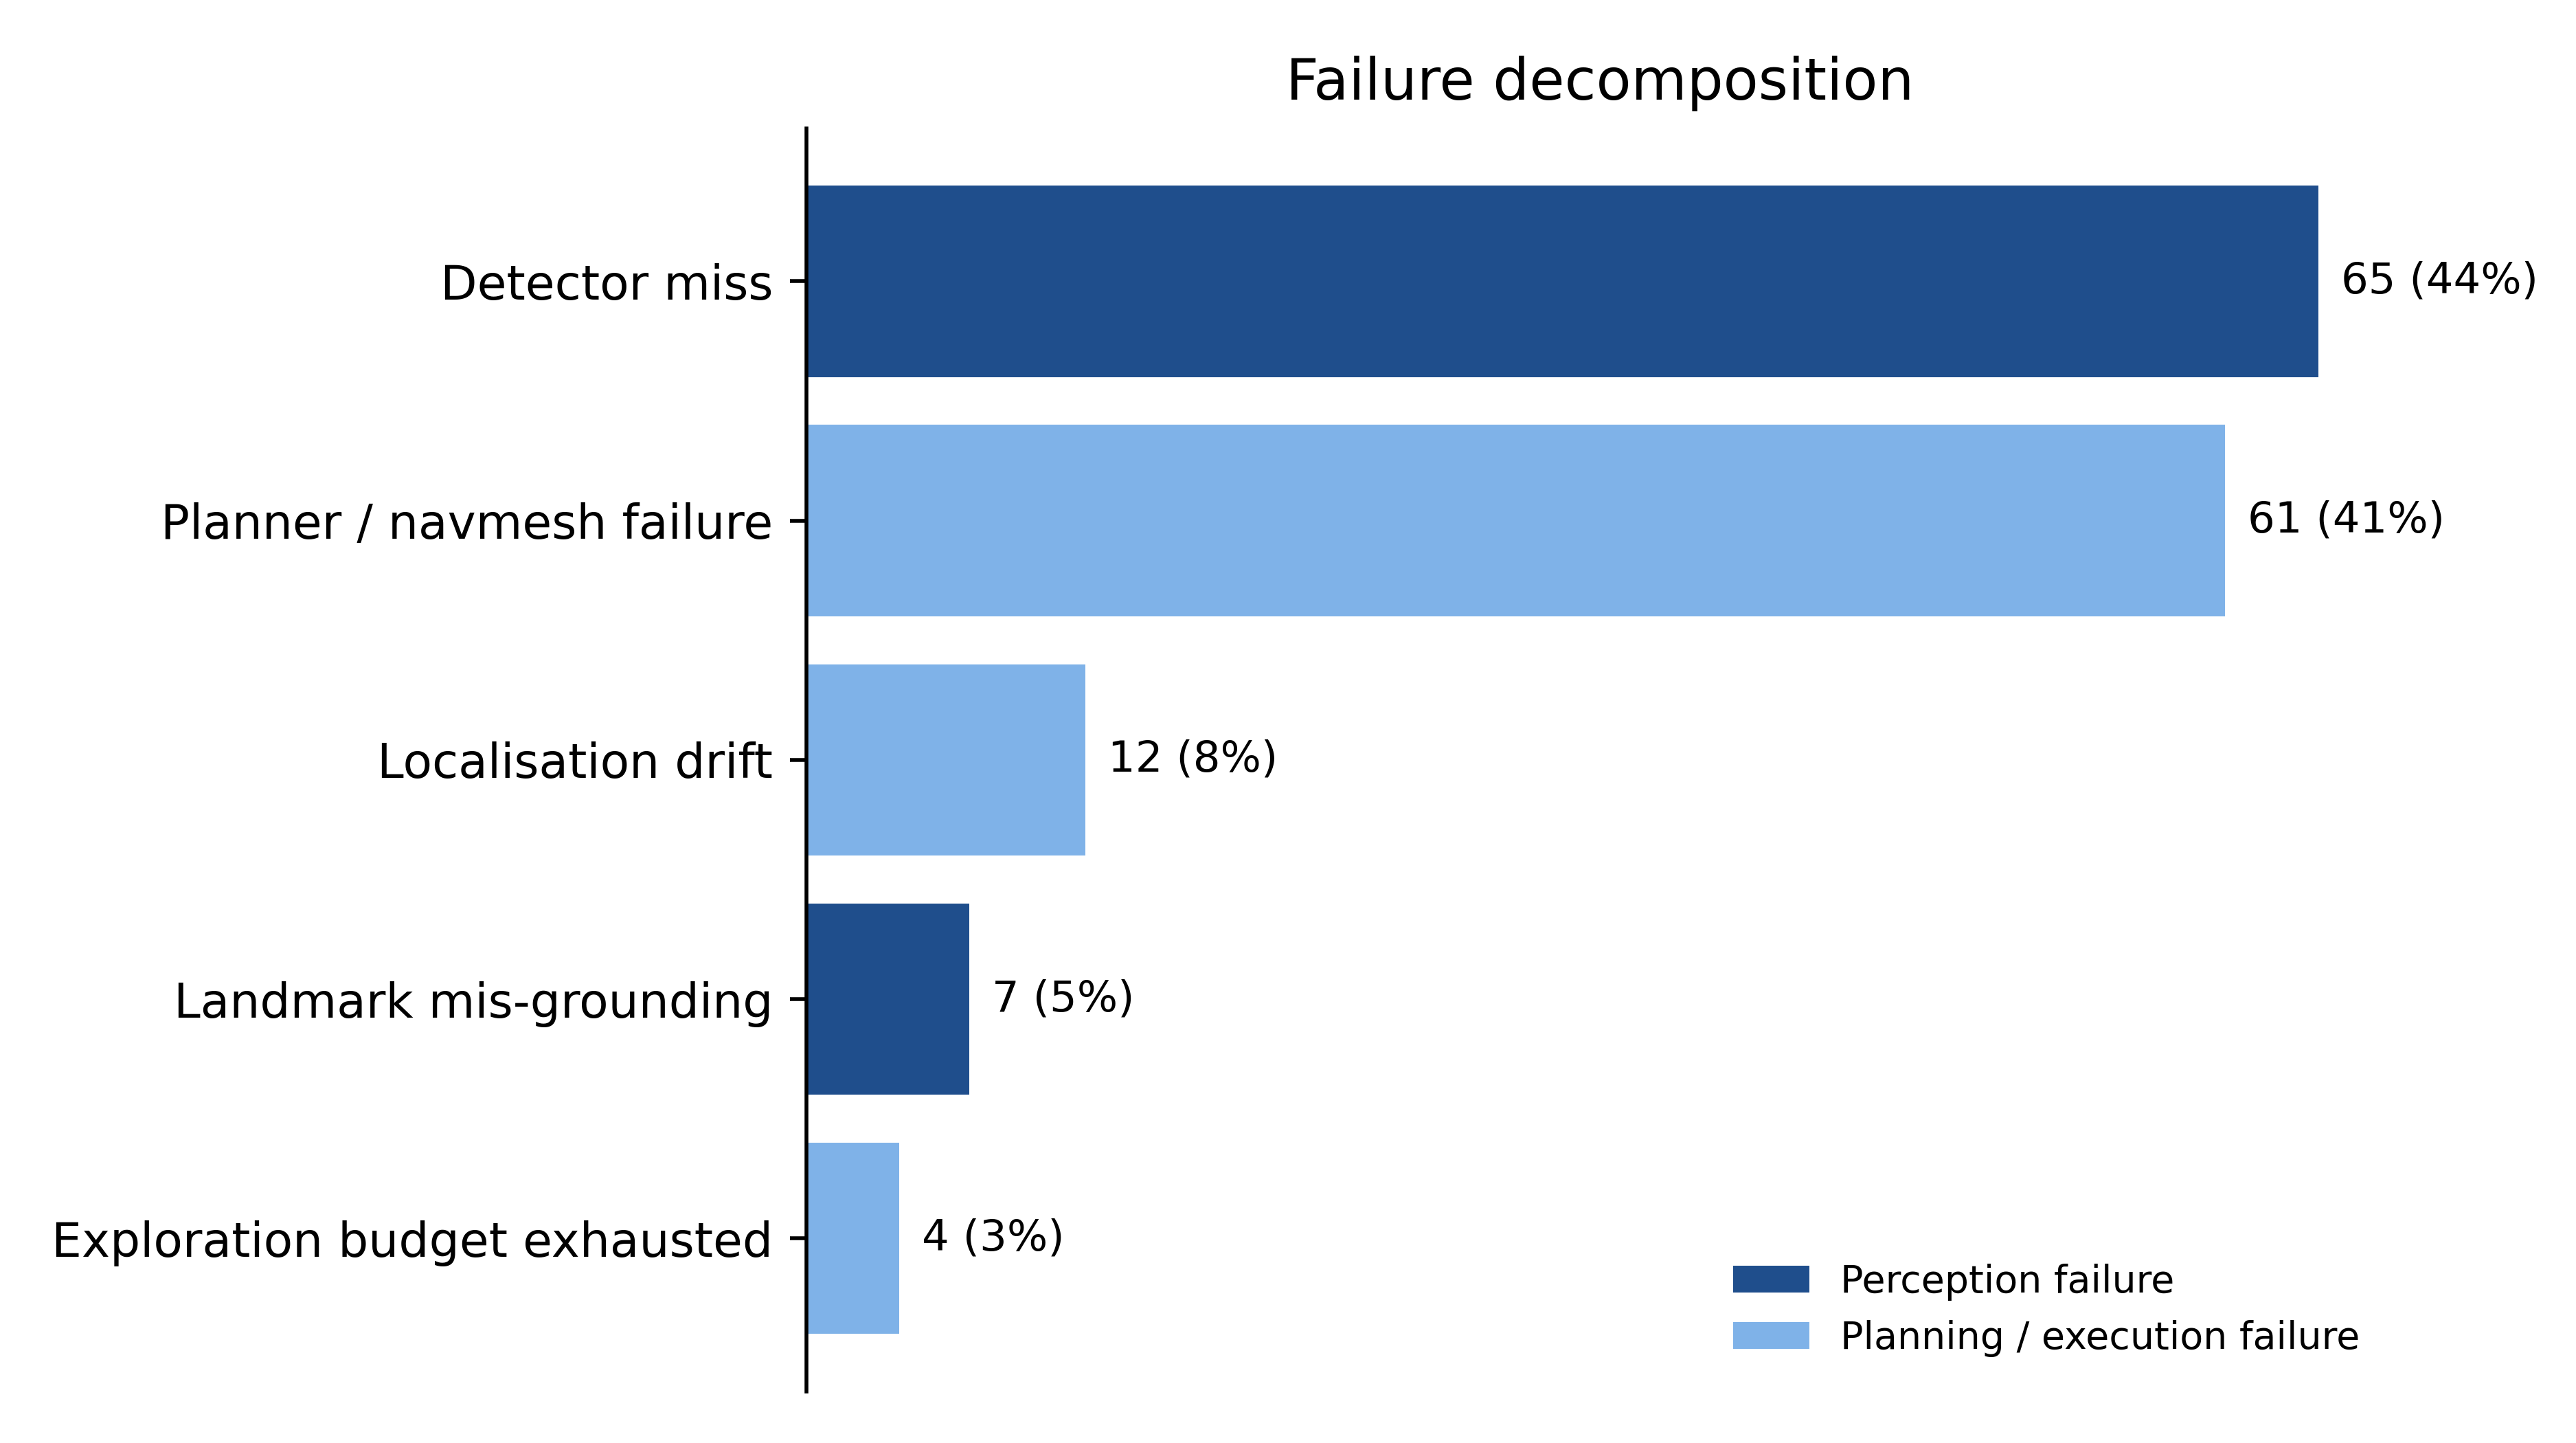
\includegraphics[width=0.88\linewidth]{figures/figure5.png}
\caption{\textbf{Failure decomposition.} By cause across $n=149$ logged records covering 19 of 32 scenes. Percentages are rounded independently and need not total 100.}
\label{fig:failures}
\end{figure}
\paragraph{Where it fails.} Figure~\ref{fig:failures} decomposes the logged subtask failures by cause, and two dominate. Detector misses account for 65 and planner or navmesh failures for 61, together 85\% of the total. Neither is addressable by better frontier selection, which bounds how much any search-side contribution can move the headline number. Figure~\ref{fig:qualitative} shows a trajectory in which surprise is high from the first corrections, the controller drops $\sigma_t$ toward its floor, and the search stays broad thereafter.

